\section{Figures} \label{sectionExample}

Figure~\ref{ExampleEstNoiseCovar}, is an example of a figure with a legend.

\begin{figure}[h]
\centering
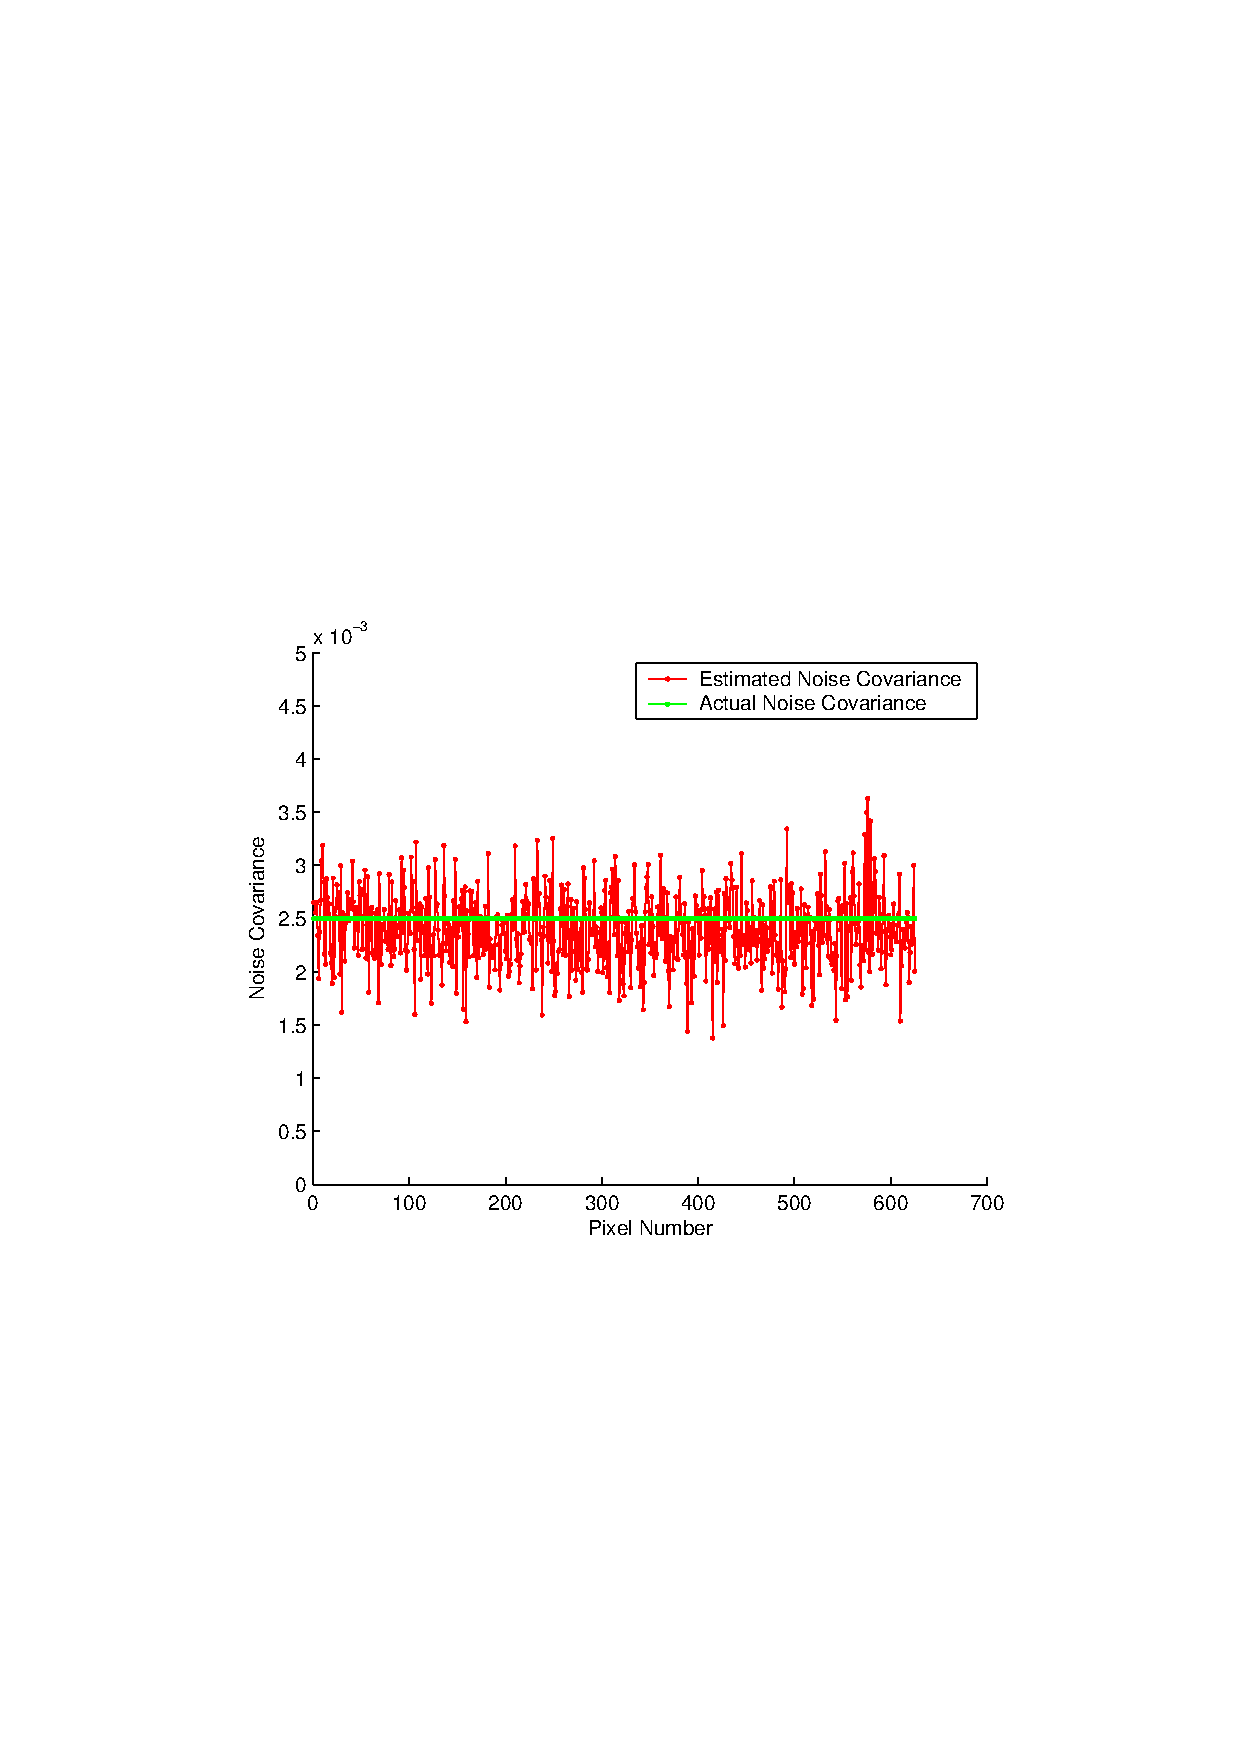
\includegraphics[width=0.5\linewidth]{exampleEstNoiseCovar}
\caption{This is the figure caption. Notice the figure looks good even when magnified because it is a vector-graphic, and not rasterized.} \label{ExampleEstNoiseCovar}
\end{figure}


\textbf{Old and New Instructions} These instructions are partly ``old'' because instead of .eps, we usually put pdf or png figures in our documents these days. However, they're still useful because exporting of Matlab figures directly to pdf, when using the Student License version of Matlab, results in an undesirable watermark. So my advice is to prepare your raster images as .png's, prepare your vector graphics as .pdf's in Inkscape or even Office (with the MS plugin that exports to .pdf), and follow the following slightly roundabout process to get Matlab figures into .pdf form.
\begin{enumerate}
  \item Make the figure in Matlab.
  \item Do \texttt{print -depsc2} to generate an .eps.
  \item Open the .eps in Ghostview (GSview) and ``Convert'' using the ``pdfwrite'' device to save a .pdf.
\end{enumerate}



\section{Test plan} \label{sec:test}

In the early stage, testing and verification of the algorithms and retrieval system are vital. While the retrieval system is completed, some test cases are also important to evaluate the performance of the system. There are several test cases: 

\begin{enumerate}[1)]
\item Retrieval test
\item Rotation invariant test
\item Noise invariant test
\item ``Scan to search'' test
\item Large database test
\end{enumerate}

The first step is to test that the retrieval system can operate correctly. A model from the model database will be input to the search engine to retrieve. The query result is expected to find the model which is exact the same as the input one from the model database. 

The second step is to verify the descriptors are correctly computed, i.e., the rotational invariance property of the descriptors is shown. A model from the model database will be loaded, and a random rotation will be applied to the model. Then the system can retrieve with the rotated model. The best result is finding out exact the same model from the database. However, due to the protential error of coefficients in rotation as well as rasterization, if the system shows models with similar shape, it is still decided as robust. 

The third step is to test the denoising module and verify the noise resistant property of the system. A model from the model database will be loaded. Certain level of noise will be added, and the denoising function can be called. Because the denoise module as well as the rasterization step cannot perfectly eliminate the noise, the system is decided as robust if the query result shows models with same or similar shapes. If these three test cases are passed, the pre-processing modules and the matching algorithm are considered to be correctly implemented. 

Afterwards, ``Scan to search'' test can be carried out. In the first place, the scanned model is loaded. Then the denoising function is called. After denoising, the system can retrieve for models with same/similar shapes. This step tests how well the matching algorithm works. And the last test is to verify the system's robustness to large database, where a large number of descriptors may have influence to the retrieval accuracy. 

\section{Results} \label{sec:results}

\begin{enumerate}
\item Retrieval test

The aim of this test is to make sure the retrieval system can operate correctly. As Figure~\ref{input_retrievaltest} and Figure~\ref{output_retrievaltest} demonstrate, the test result shows every module of the retrieval system is correctly implemented, and the models in the database can be searched. 

\begin{figure}[h]
\centering
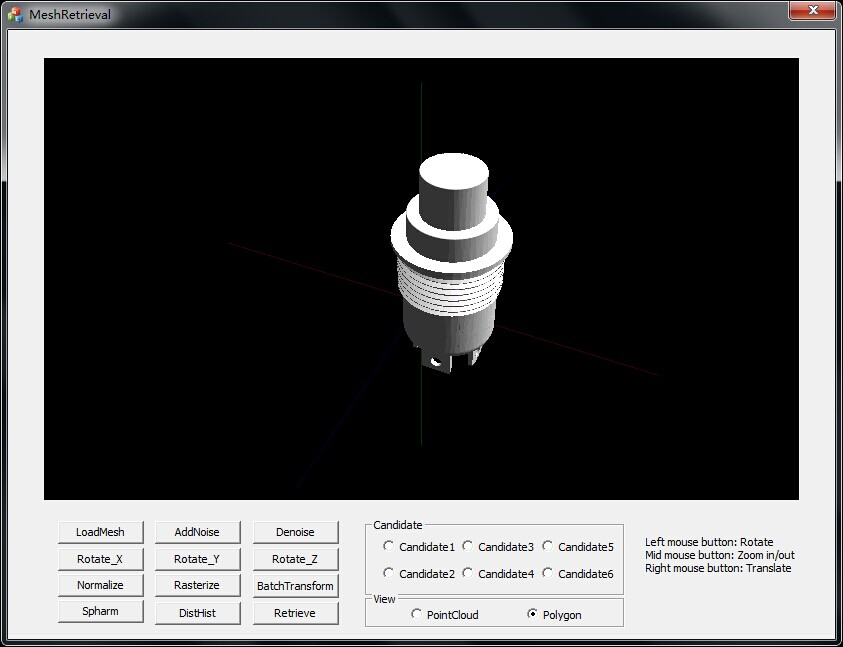
\includegraphics[width=0.7\linewidth]{input_initialdesign}
\caption{Input of the retrieval test} \label{input_retrievaltest}
\end{figure}

\begin{figure}[h]
\centering
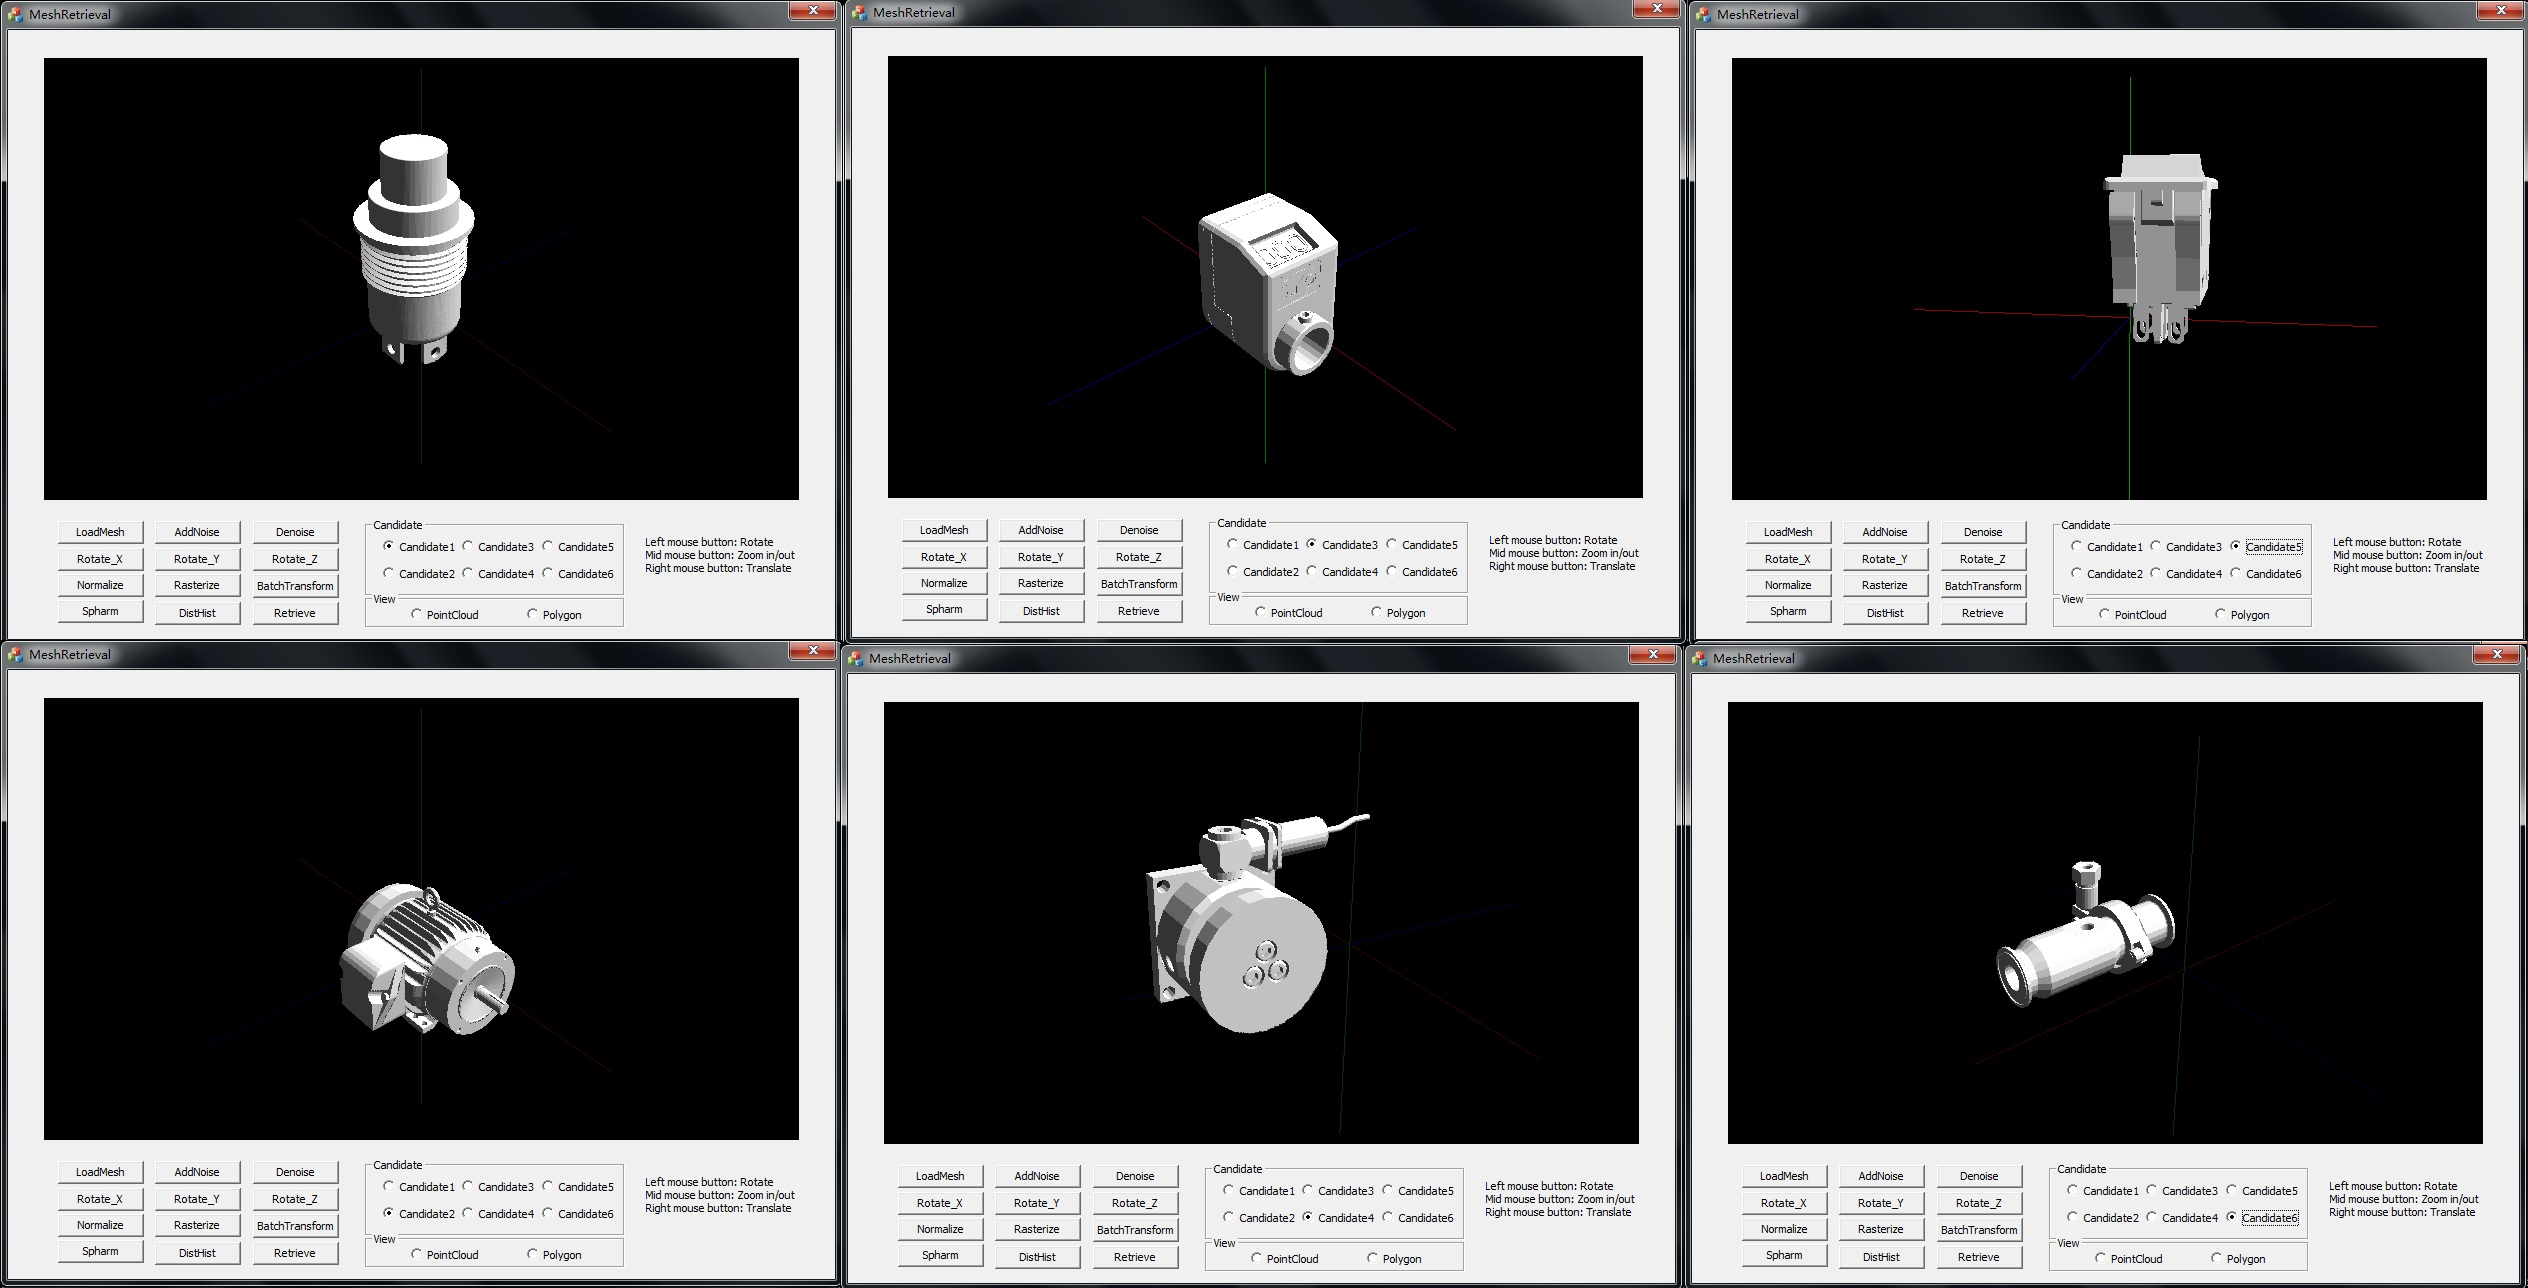
\includegraphics[width=0.7\linewidth]{output_finaldesign}
\caption{Output of the retrieval test} \label{output_retrievaltest}
\end{figure}

\item Rotation invariant test

In this test, rotational invariance property is verified. Firstly, a normal model with cylinder shape is input (Figure~\ref{input_rotationinvariant_test10}). The retrieval result is demonstated in Figure~\ref{output_rotationinvariant_test10}. Then a model with unusual flat shape is input to test the robustness of the descriptors. Figure~\ref{input_rotationinvariant_test32} and Figure~\ref{output_rotationinvariant_test32} demonstrate the input and output. For both of these two tests, it can be noticed that the input model is rotated to a random direction, and the first candidate (with the highest similarity) of the output is exactly the same as the input model. 

\begin{figure}[h]
\centering
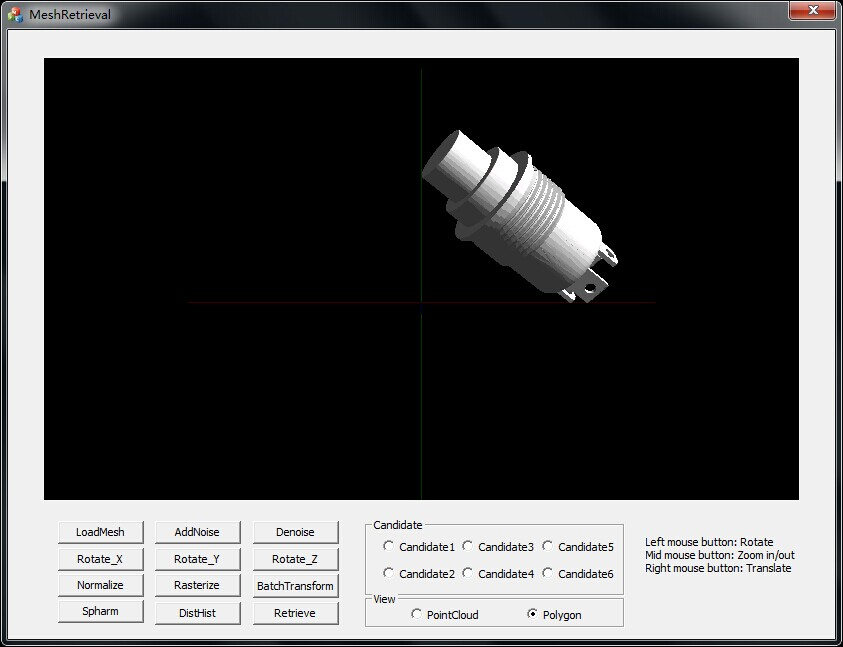
\includegraphics[width=0.7\linewidth]{input_rotationinvariant_test10}
\caption{Input model of the retrieval test. It is rotated to a random direction} \label{input_rotationinvariant_test10}
\end{figure}

\begin{figure}[h]
\centering
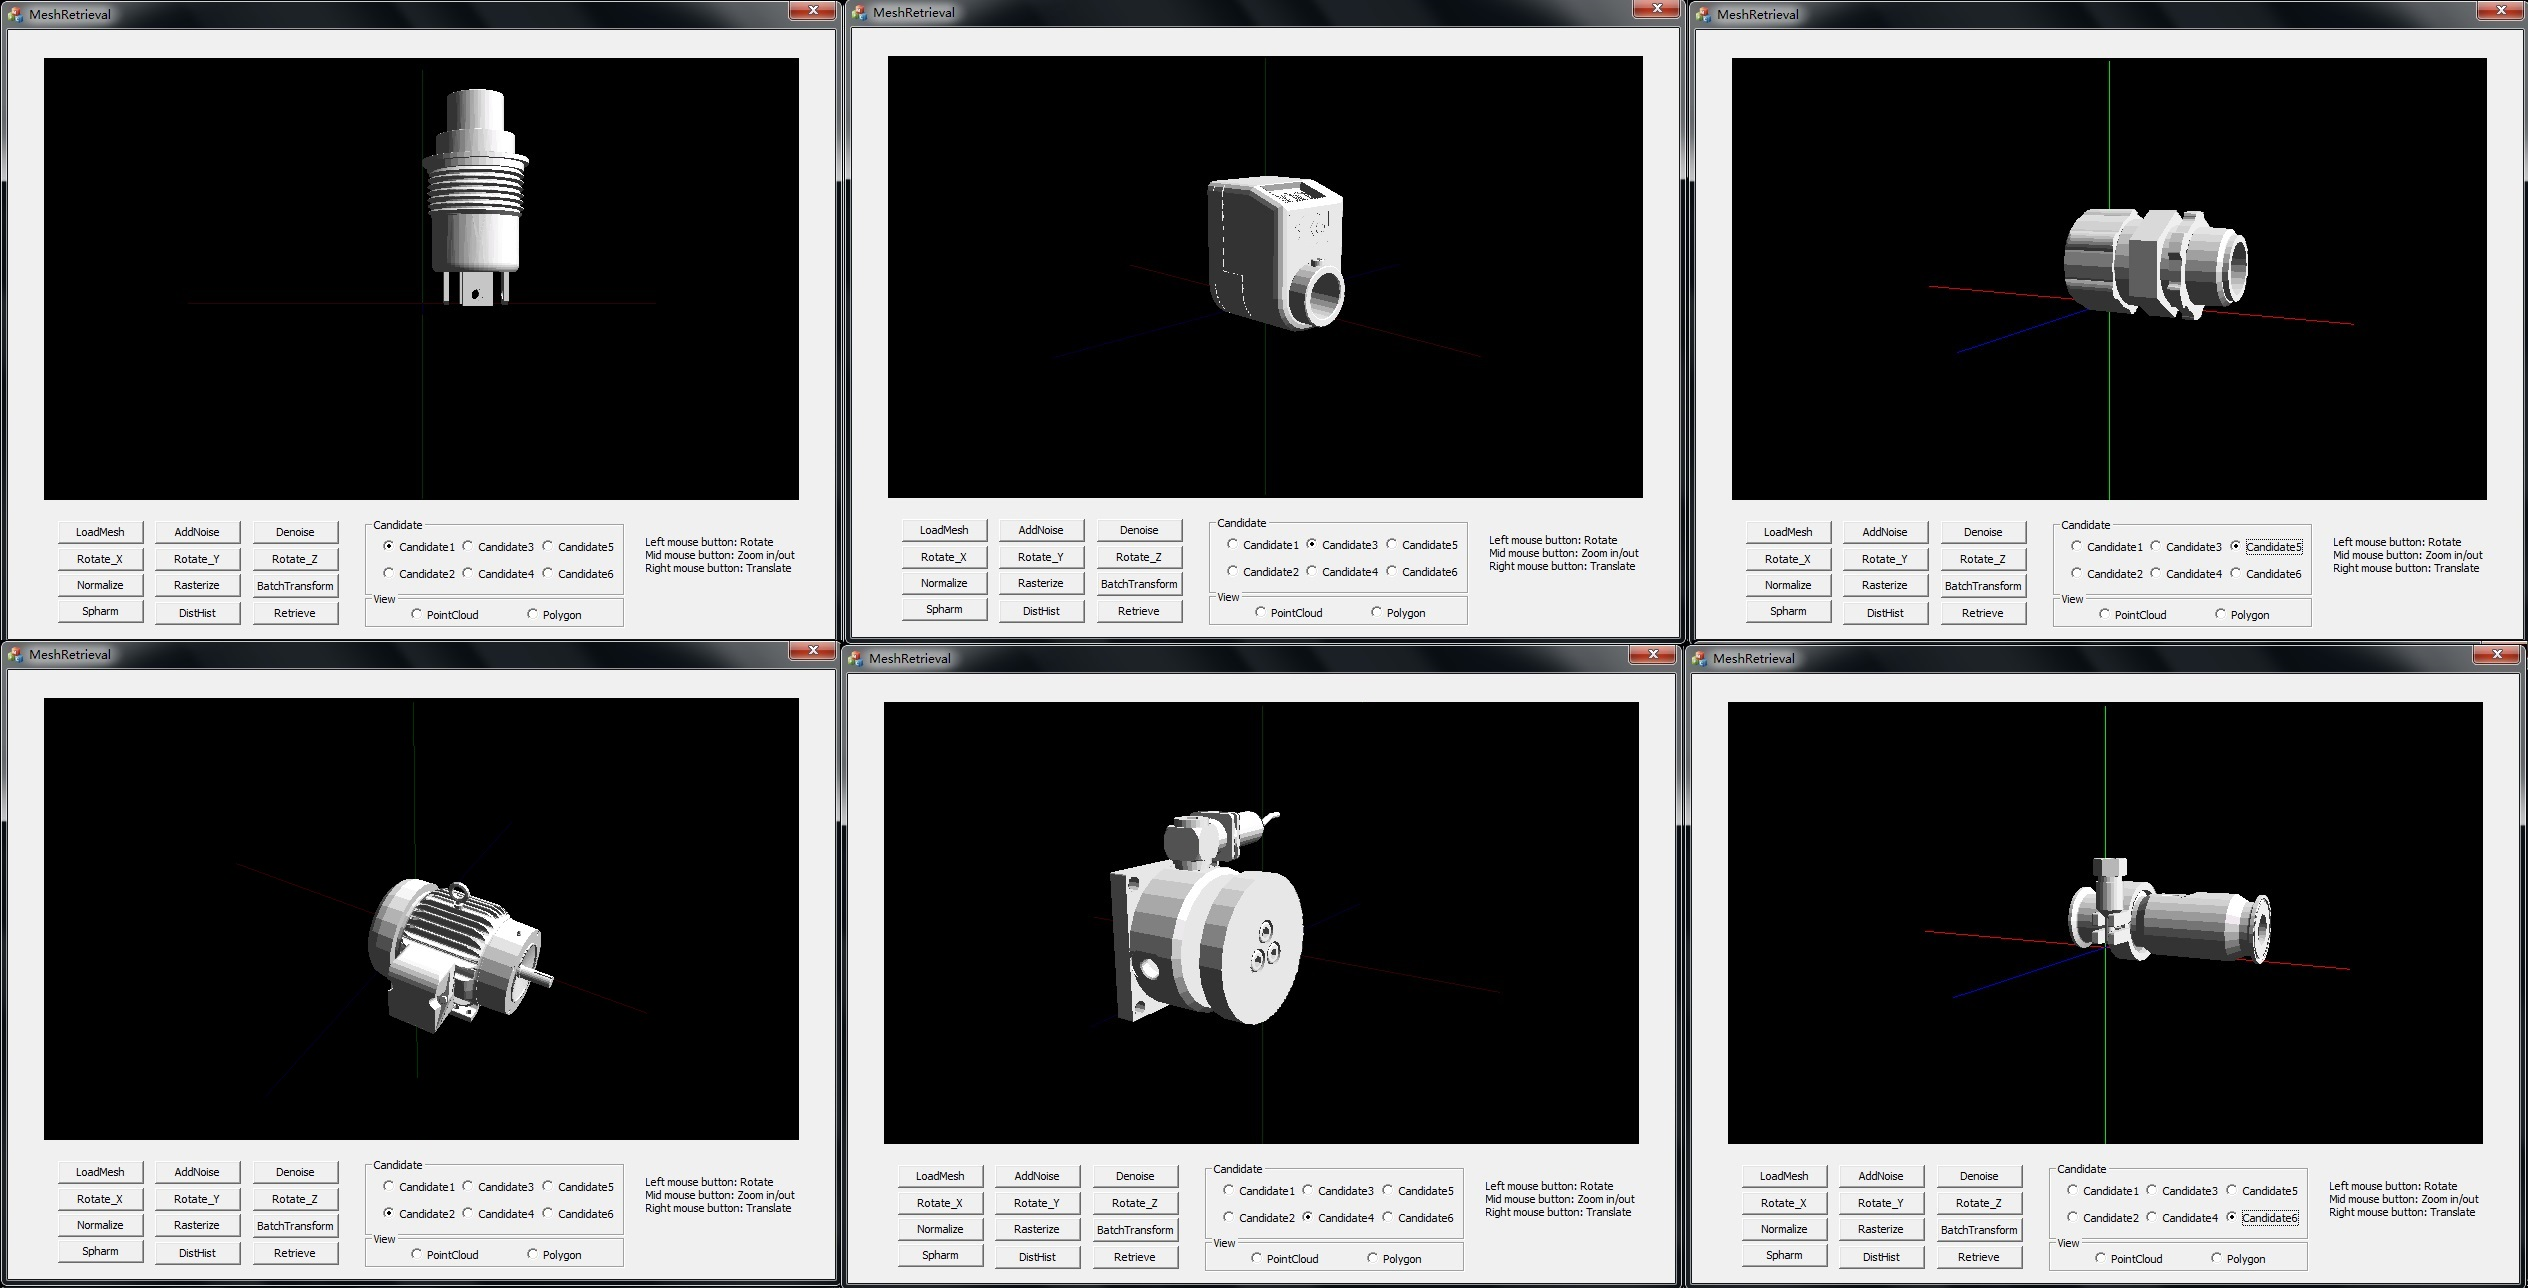
\includegraphics[width=0.7\linewidth]{output_rotationinvariant_test10}
\caption{Output of the retrieval test. The first candidate (with the highest similarity) is exactly the same as the input model} \label{output_rotationinvariant_test10}
\end{figure}

\begin{figure}[h]
\centering
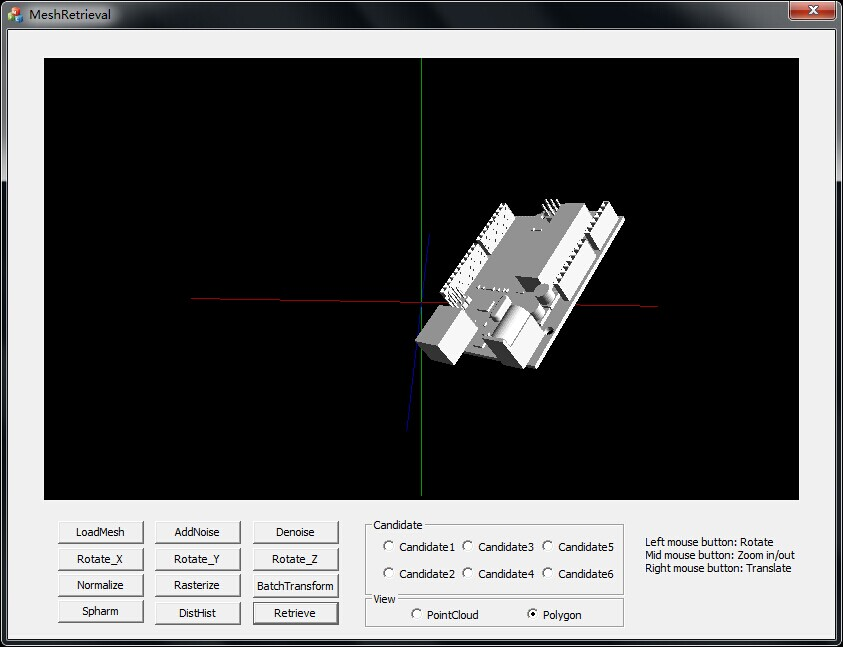
\includegraphics[width=0.7\linewidth]{input_rotationinvariant_test32}
\caption{Input model of the retrieval test. It is rotated to a random direction} \label{input_rotationinvariant_test32}
\end{figure}

\begin{figure}[h]
\centering
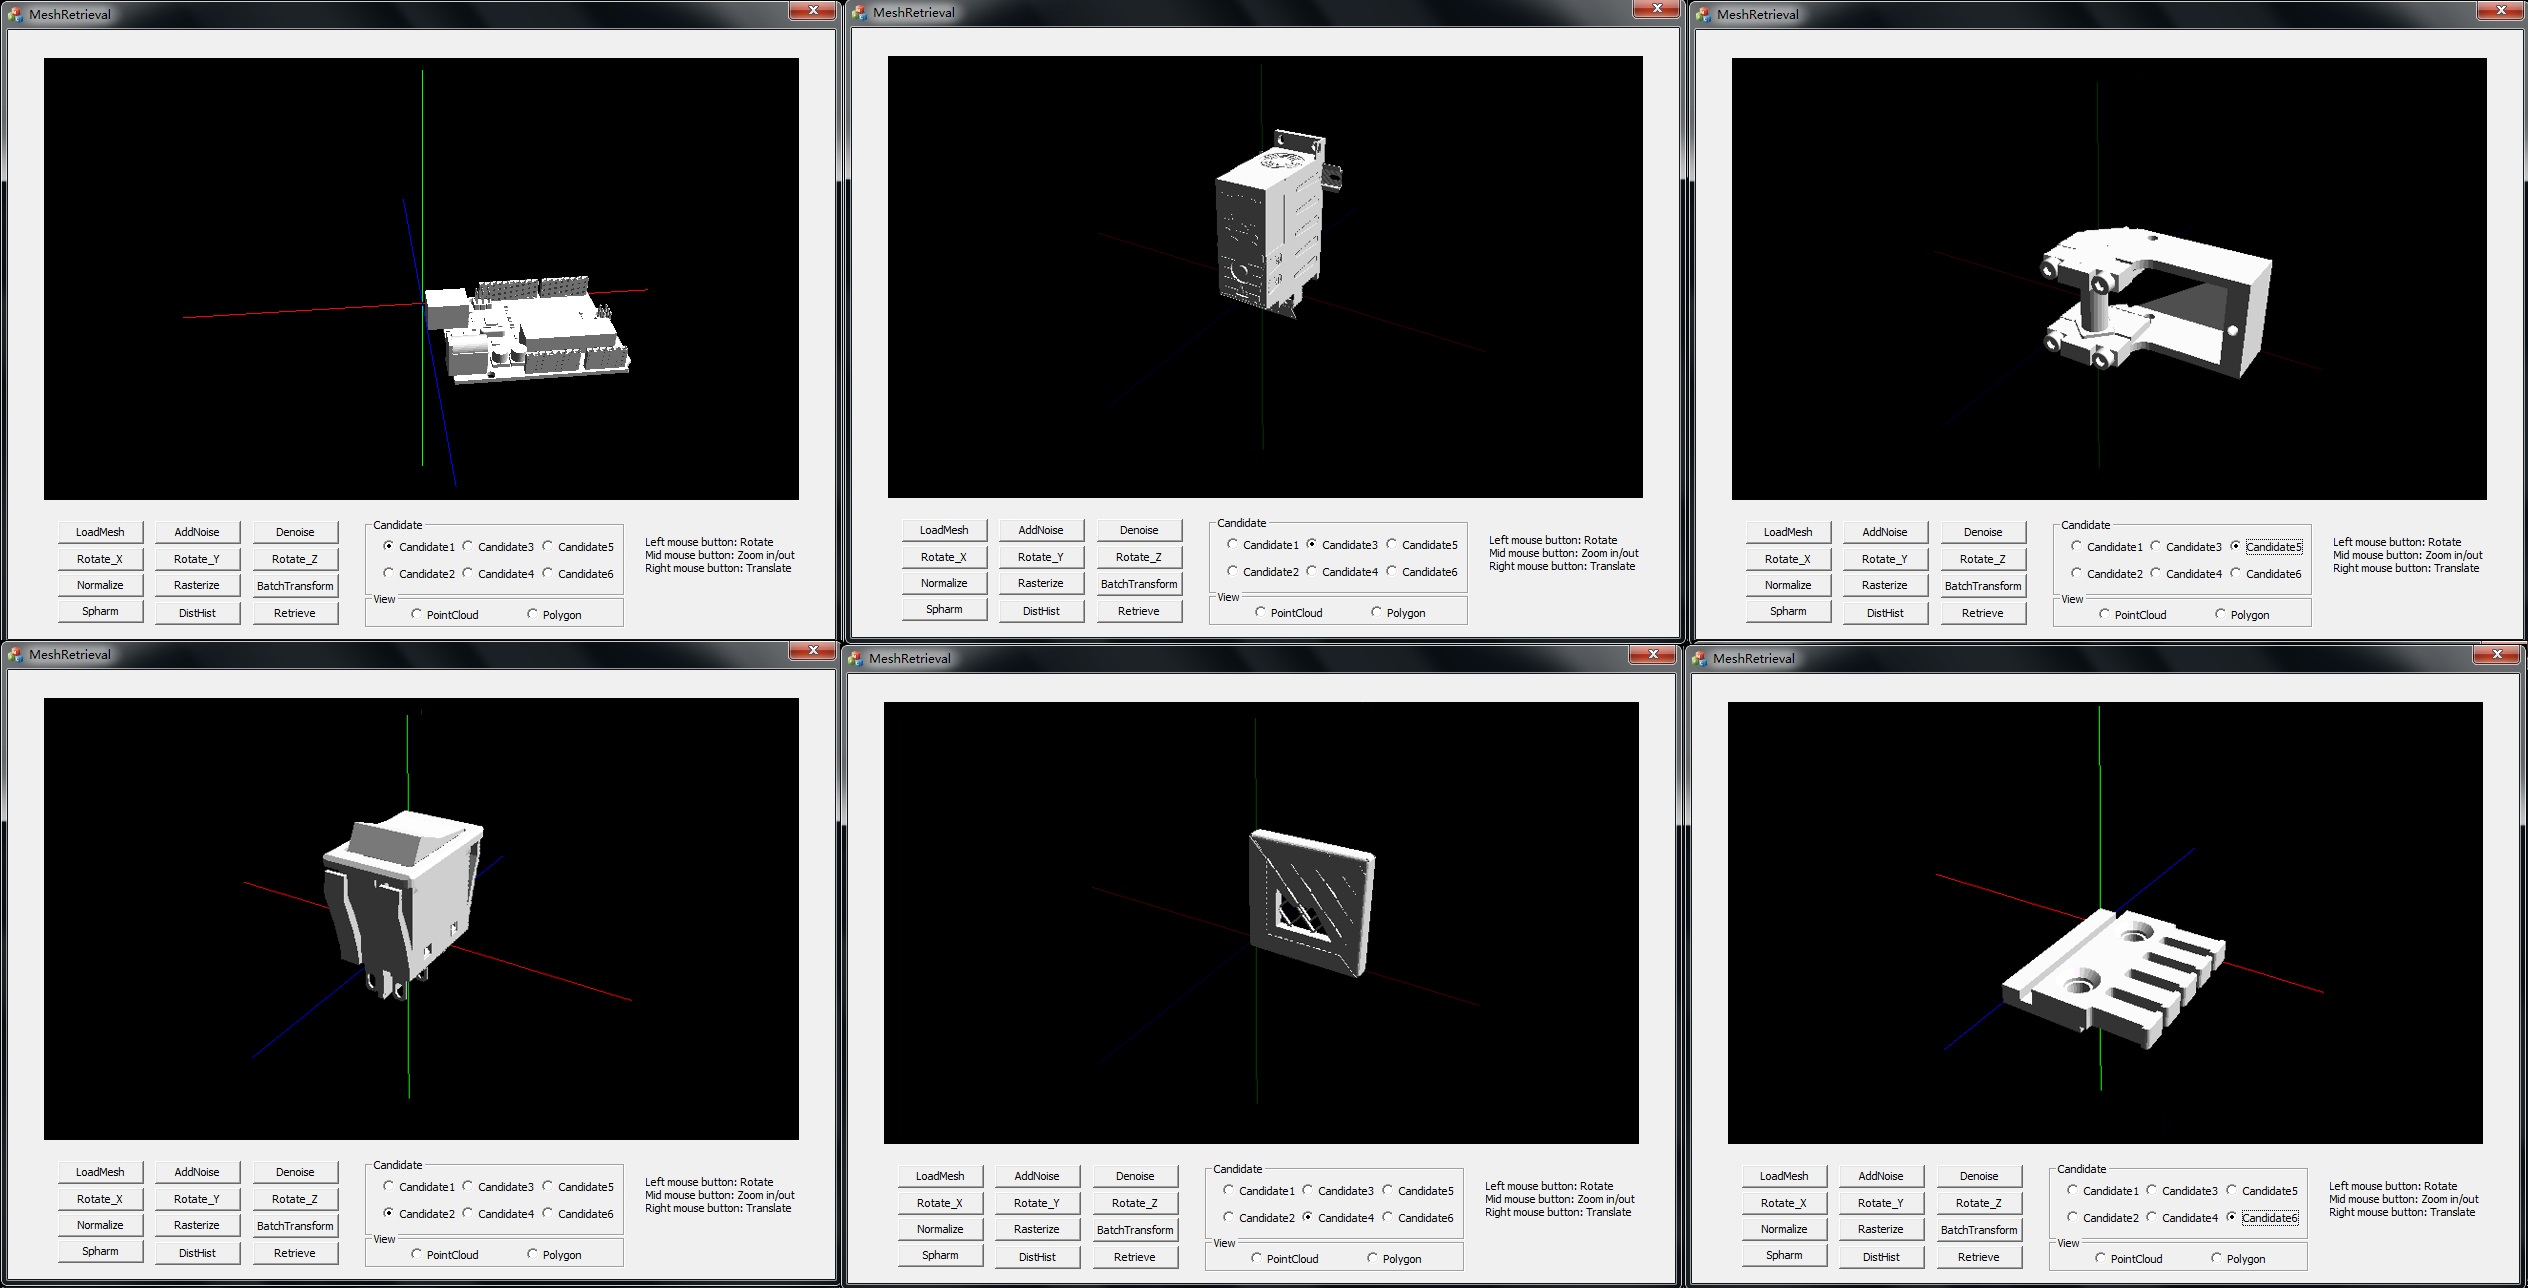
\includegraphics[width=0.7\linewidth]{output_rotationinvariant_test32}
\caption{Output of the retrieval test. The first candidate (with the highest similarity) is exactly the same as the input model} \label{output_rotationinvariant_test32}
\end{figure}

The descriptors:

\begin{figure}[h]
\centering
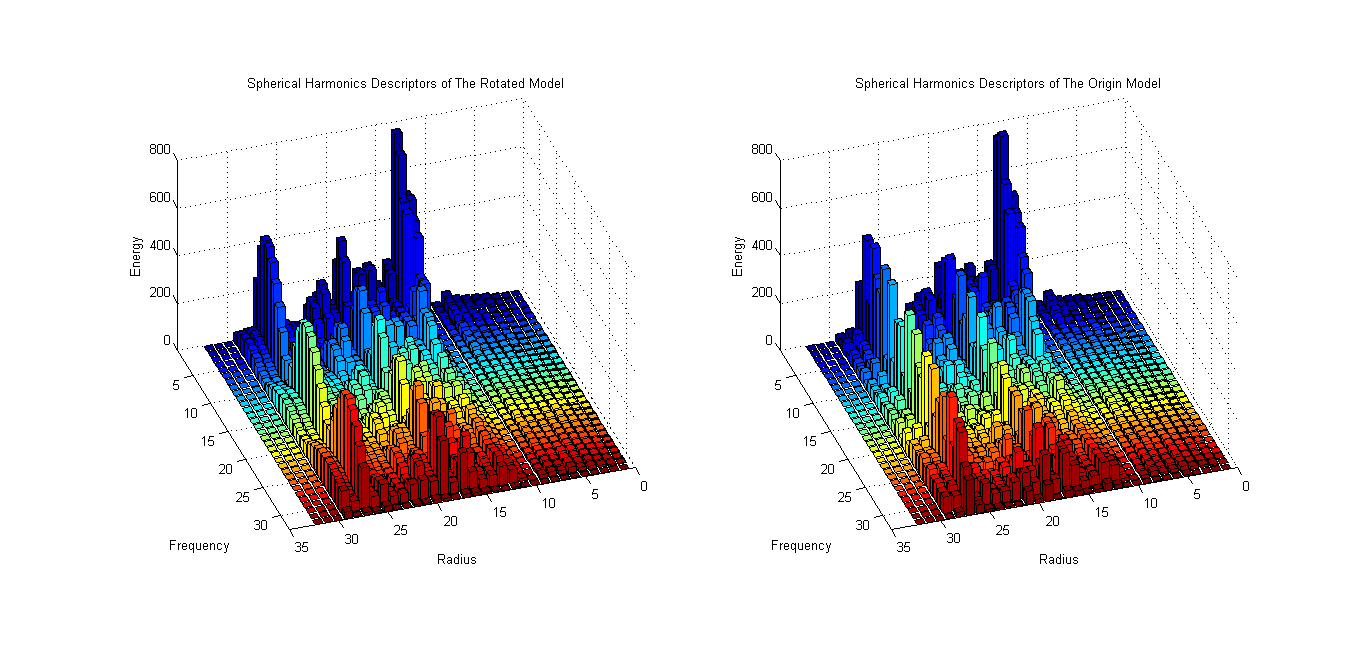
\includegraphics[width=0.7\linewidth]{rotationinvariant_test_SH10}
\caption{a} \label{rotationinvariant_test_SH10}
\end{figure}

\begin{figure}[h]
\centering
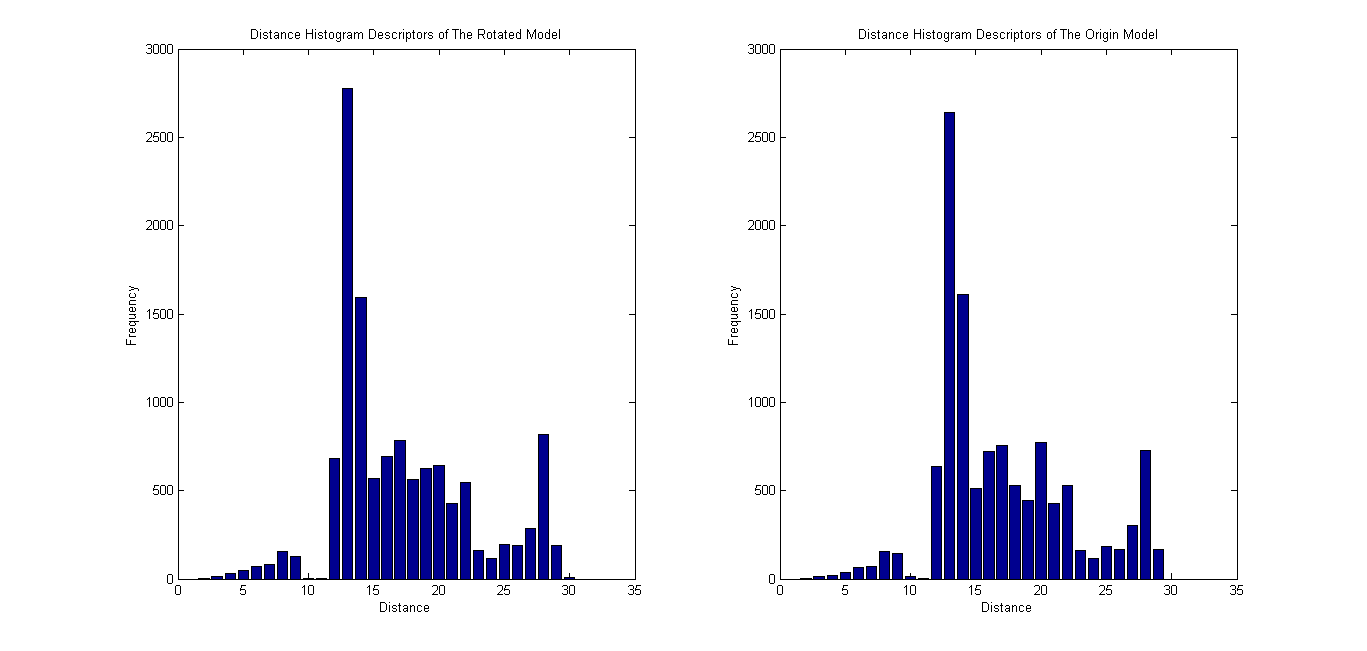
\includegraphics[width=0.7\linewidth]{rotationinvariant_test_DH10}
\caption{a} \label{rotationinvariant_test_DH10}
\end{figure}

\begin{figure}[h]
\centering
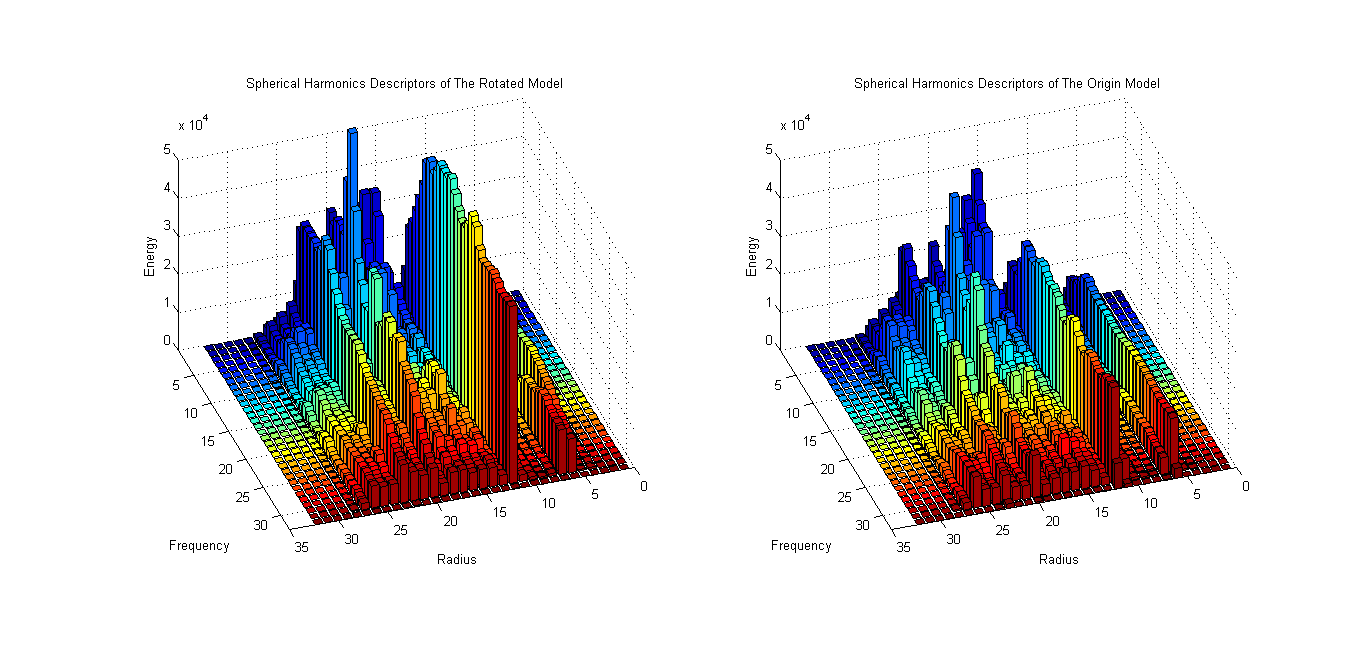
\includegraphics[width=0.7\linewidth]{rotationinvariant_test_SH32}
\caption{a} \label{rotationinvariant_test_SH32}
\end{figure}

\begin{figure}[h]
\centering
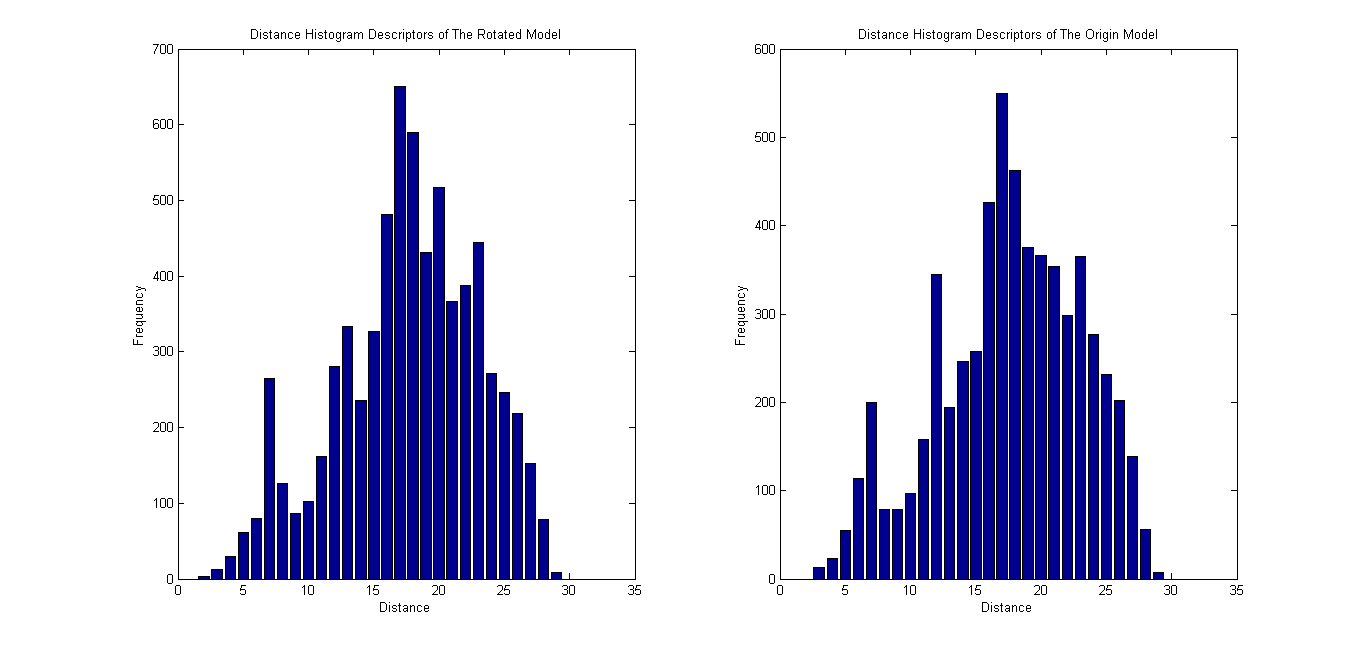
\includegraphics[width=0.7\linewidth]{rotationinvariant_test_DH32}
\caption{a} \label{rotationinvariant_test_DH32}
\end{figure}



SH  DH   vs SH DH

Noise invariant test
INPUT UI
OUTPUT UI
SH  DH   vs SH DH

``Scan to search'' test 
INPUT UI
OUTPUT UI
SH  DH   vs   SH DH

Large database test
NO FIGURES
In the initial design, there is only one spherical harmonics descriptors. And a single type of descriptors may have its weakness. Due to some unknown errors in the descriptors (maybe it is the rasterization error or sampling error in the spherical harmonics transformation), there are sometimes some irrelevant matches. This is analysed in Section~\ref{sec:thefinaldesign}.  Also as test result suggests, another type of descriptors (distance histogram) is added for assistance. 

\end{enumerate}
